\chapter{Preliminaries, Background, and Evaluation Metrics}
\label{ch:background}



\vspace{0.5em}
\noindent\rule{\textwidth}{0.4pt}
\textbf{Declaration of Contributions:} 
    \begin{itemize}[leftmargin=*,noitemsep]
    \item \textbf{Siddharth Gupta} — was responsible for the sections on representation learning, including autoencoders, variational autoencoders, disentangled representations, and related architectural foundations.
    \item \textbf{Aryan Choudhary} — contributed the development and formalisation of the Conditional Value-at-Risk (CVaR) framework and its role in fairness-aware optimisation. 
    \item \textbf{Vishesh Gupta} — designed and documented the evaluation metrics, including fairness and performance measures such as Equal Opportunity, Equalized Odds, and FPR-based metrics.
    \end{itemize}
\noindent\rule{\textwidth}{0.4pt}
\vspace{1em}

This chapter lays the conceptual and mathematical groundwork required
to understand the fairness-aware machine-learning techniques surveyed
in subsequent chapters.  We begin with the essential mathematical
building blocks—drawing on analysis and probability—then introduce the
AI/ML architectures that appear throughout the literature, and finally
define the fairness metrics used to quantify bias.

% , , , , , , , , , , , , , , , , , , , , , , 
\section{Mathematical Foundations}
\label{sec:math_foundations}
% , , , , , , , , , , , , , , , , , , , , , , 

\subsection{Sets, Functions, and Notation}
\label{subsec:notation}

Throughout this report we adopt the following notation.
Scalars are denoted by lower-case italic letters ($x, y, z$);
vectors by bold lower-case ($\mathbf{x}, \mathbf{z}$); and
matrices by bold upper-case ($\mathbf{W}, \mathbf{X}$).
The set of real numbers is $\mathbb{R}$, and $\mathbb{R}^d$ denotes
a $d$-dimensional real vector space.  We write

$\mathcal{X}$ for an input space and $\mathcal{Z}$ for a latent
(hidden) space.

A \emph{random variable} $X$ defined over a probability space
$(\Omega,\mathcal{F},\mathbb{P})$ takes values in $\mathcal{X}$.
Its \emph{probability distribution} is denoted $P_X$ or simply $P$.
The \emph{expectation} of a function $f(X)$ is
\[
  \mathbb{E}_{X \sim P}\bigl[f(X)\bigr]
  \;=\; \int_{\mathcal{X}} f(x)\,\mathrm{d}P(x).
\]

\subsection{Infimum and Supremum}
\label{subsec:inf_sup}

Two operations appear repeatedly in the loss functions of the papers
we review.

\begin{itemize}
  \item The \textbf{infimum} ($\inf$) of a set $S \subseteq \mathbb{R}$
        is its \emph{greatest lower bound}: the largest value $\ell$
        such that $s \geq \ell$ for every $s \in S$.  For a
        function $f:\Lambda \to \mathbb{R}$ we write
        $\inf_{\lambda \in \Lambda} f(\lambda)$ to mean
        the smallest value $f$ can approach (not necessarily attained).
  \item The \textbf{supremum} ($\sup$) is the \emph{least upper bound},
        analogously defined.
\end{itemize}

\noindent
These concepts are essential when the minimum or maximum of a
function is not attained—a situation that arises naturally in
risk-based fairness objectives (see Section~\ref{sec:cvar}).

\subsection{Kullback-Leibler Divergence}
\label{subsec:kl}

Given two probability distributions $P$ and $Q$ over the same space,
the \emph{Kullback–Leibler (KL) divergence} measures how much $P$
diverges from $Q$:
\begin{equation}
  D_{\mathrm{KL}}(P \| Q)
  \;=\; \mathbb{E}_{x \sim P}
        \!\left[\log \frac{P(x)}{Q(x)}\right]
  \;=\; \int P(x)\,\log \frac{P(x)}{Q(x)}\,\mathrm{d}x.
  \label{eq:kl_divergence}
\end{equation}
$D_{\mathrm{KL}}(P \| Q) \geq 0$ always, with equality iff $P = Q$
almost everywhere.  KL divergence is \emph{asymmetric}: in general
$D_{\mathrm{KL}}(P\|Q) \neq D_{\mathrm{KL}}(Q\|P)$.

\noindent\textbf{Role in VAEs.}
In Variational Autoencoders (Section~\ref{sec:vae}), the KL divergence
acts as a regulariser that pushes the approximate posterior
$q_\Phi(\mathbf{z}|\mathbf{x})$ towards the standard Gaussian prior
$p(\mathbf{z}) = \mathcal{N}(\mathbf{0}, \mathbf{I})$.

\subsection{Total Correlation}
\label{subsec:tc}

\emph{Total Correlation} (TC), introduced by Watanabe
\cite{watanabe1960}, generalises mutual information to measure the
overall statistical dependency among $n$ random variables
$z_1, z_2, \ldots, z_n$:
\begin{equation}
  \mathrm{TC}(z_1, \ldots, z_n)
  \;=\; D_{\mathrm{KL}}\!\left(
        q(z_1, z_2, \ldots, z_n)
        \;\Big\|\;
        \prod_{j=1}^{n} q(z_j)
        \right).
  \label{eq:total_correlation}
\end{equation}
When TC equals zero, all variables are mutually independent.
Minimising TC during training therefore encourages a model to learn
representations whose components carry non-overlapping information—the
core idea behind \emph{disentangled} representation learning
(Section~\ref{sec:disentangled}).

\subsection{Mutual Information}
\label{subsec:mutual_info}

The \emph{mutual information} between two random variables $X$ and $Y$
quantifies how much knowing $X$ reduces uncertainty about $Y$:
\begin{equation}
  I(X; Y)
  \;=\; D_{\mathrm{KL}}\bigl(P_{XY} \| P_X \otimes P_Y\bigr)
  \;=\; \mathbb{E}_{(x,y)\sim P_{XY}}
        \!\left[\log \frac{P_{XY}(x,y)}{P_X(x)\,P_Y(y)}\right].
  \label{eq:mutual_info}
\end{equation}
In fair representation learning, we want the encoded features
$\mathbf{z}$ to have \emph{high} mutual information with the input
$\mathbf{x}$ (to preserve utility) but \emph{low} mutual information
with a sensitive attribute $s$ (to ensure fairness).

\subsection{Evidence Lower Bound (ELBO)}
\label{subsec:elbo}

Exact marginal likelihood $\log p_\Theta(\mathbf{x})$ is
intractable for deep latent-variable models.
Jensen's inequality gives a tractable surrogate known as
the \textbf{Evidence Lower BOund (ELBO)}:
\begin{equation}
  \log p_\Theta(\mathbf{x})
  \;\geq\;
  \underbrace{%
    \mathbb{E}_{q_\Phi(\mathbf{z}|\mathbf{x})}\!
    \bigl[\log p_\Theta(\mathbf{x}|\mathbf{z})\bigr]
  }_{\text{reconstruction term}}
  \;-\;
  \underbrace{%
    D_{\mathrm{KL}}\!\bigl(
      q_\Phi(\mathbf{z}|\mathbf{x})
      \;\|\;
      p(\mathbf{z})
    \bigr)
  }_{\text{regularisation term}}
  \;=:\; \mathcal{L}_{\mathrm{VAE}}.
  \label{eq:elbo}
\end{equation}
Maximising $\mathcal{L}_{\mathrm{VAE}}$ simultaneously encourages
faithful reconstruction and a well-behaved latent distribution.

\subsection{Conditional Value-at-Risk (CVaR)}
\label{sec:cvar}

Standard empirical risk minimisation (ERM) minimises the
\emph{average} loss:
\begin{equation}
  \mathcal{R}_{\mathrm{avg}}(\theta)
  \;:=\; \mathbb{E}_{(X,Y)\sim P}\!\bigl[\ell(\theta;\,X,Y)\bigr].
  \label{eq:erm}
\end{equation}
Because the average is dominated by easy (majority) samples, ERM
tends to underperform on rare demographic subgroups—precisely the
fairness problem.  \emph{Distributionally Robust Optimisation} (DRO)
addresses this by minimising the \emph{worst-case} risk
$\mathcal{R}_{\max}(\theta) = \max_m \mathbb{E}_{(X,Y)\sim P_m}
[\ell(\theta;X,Y)]$ over unknown latent groups.

A tractable upper bound on $\mathcal{R}_{\max}$ is given by
\emph{Conditional Value-at-Risk} at level $\alpha \in (0,1)$
\cite{rockafellar2000}:
\begin{equation}
  \mathrm{CVaR}_{\alpha}(\theta)
  \;:=\; \inf_{\lambda \in \mathbb{R}}
         \left\{
           \lambda
           + \frac{1}{\alpha}\,
           \mathbb{E}_{(X,Y)\sim P}\!
           \bigl[\ell(\theta;\,X,Y) - \lambda\bigr]_{+}
         \right\},
  \label{eq:cvar1}
\end{equation}
where $[a]_{+} = \max\{0,a\}$ is the hinge (ReLU) function.
\begin{figure}[!htbp]
  \centering
  % , - TikZ figure: ERM vs CVaR loss landscape , -
  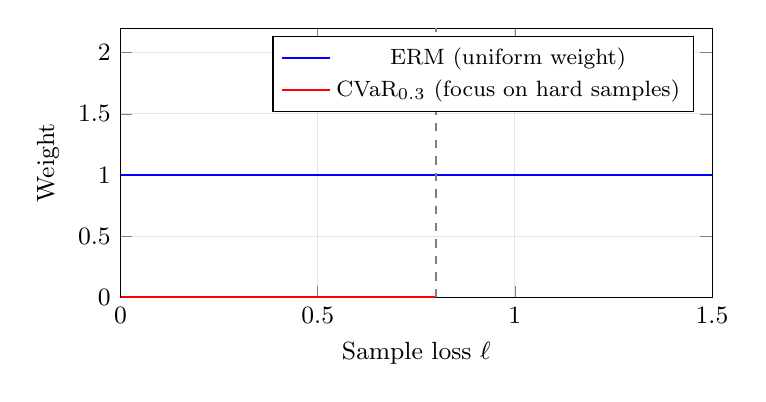
\begin{tikzpicture}[font=\small]
    \begin{axis}[
        width=0.75\textwidth, height=5cm,
        xlabel={Sample loss $\ell$},
        ylabel={Weight},
        xmin=0, xmax=1.5,
        ymin=0, ymax=2.2,
        xtick={0,0.5,1,1.5},
        ytick={0,0.5,1,1.5,2},
        legend style={at={(0.97,0.97)},anchor=north east,
                      font=\footnotesize},
        grid=major, grid style={gray!20},
    ]
      %% ERM: flat weighting
      \addplot[blue, thick, domain=0:1.5]{1};
      \addlegendentry{ERM (uniform weight)}

      %% CVaR: zero below lambda, 1/alpha above
      \addplot[red, thick, domain=0:0.8]{0};
      \addplot[red, thick, domain=0.8:1.5]{1/0.3};
      \addlegendentry{CVaR$_{0.3}$ (focus on hard samples)}

      %% lambda marker
      \draw[dashed,gray] (axis cs:0.8,0) -- (axis cs:0.8,2.2)
            node[above,gray]{$\lambda^*$};
    \end{axis}
  \end{tikzpicture}
  \caption{Comparison of sample weighting under ERM and CVaR at
           $\alpha = 0.3$.  ERM weights all samples uniformly,
           whereas CVaR assigns zero weight to easy samples
           (loss $< \lambda^*$) and amplified weight to hard
           samples (loss $> \lambda^*$).  Minimising CVaR therefore
           focuses training on the worst-performing subgroups.}
  \label{fig:cvar_weighting}
\end{figure}

\noindent
\textbf{Proposition} (Proposition~1 in \cite{ju2024}).
\emph{If each latent group $m$ occurs with probability
$\pi_m \geq \alpha$, then
$\mathrm{CVaR}_\alpha(\theta) \geq \mathcal{R}_{\max}(\theta)$.}
Hence minimising CVaR minimises an upper bound on the worst-case
group risk.

\noindent\textbf{Group-level CVaR.}
When demographic labels are available, one can apply CVaR at
the group level:
\begin{equation}
  \mathrm{CVaR}^{\mathcal{G}}_{\alpha}(\theta)
  \;:=\; \inf_{\lambda \in \mathbb{R}}
         \left\{
           \lambda
           + \frac{1}{\alpha}\,
           \mathbb{E}_{G \sim \mathrm{Uniform}(\mathcal{G})}
           \bigl[\mathcal{R}_G(\theta) - \lambda\bigr]_{+}
         \right\},
  \label{eq:group_cvar1}
\end{equation}
where $\mathcal{R}_G(\theta)$ is the per-group risk.  This formulation
simultaneously minimises average group risk and minimises the
disparity across groups \cite{williamson2019}.

% , , , , , , , , , , , , , , , , , , , , , , 
\section{Representation Learning}
\label{sec:repr_learning}
% , , , , , , , , , , , , , , , , , , , , , , 

\emph{Representation learning} is the subfield of machine learning
concerned with automatically discovering compact, informative
features (representations) from raw data \cite{bengio2013}.
Rather than hand-crafting features, a model—typically a deep neural
network—learns a function $f_\theta: \mathcal{X} \to \mathcal{Z}$
that maps high-dimensional inputs $\mathbf{x}$ to a
lower-dimensional \emph{latent} (embedding) vector $\mathbf{z}$.
The key desiderata are:

\begin{enumerate}
  \item \textbf{Informativeness}: $\mathbf{z}$ retains enough
        information about $\mathbf{x}$ for downstream tasks.
  \item \textbf{Compactness}: $\mathbf{z}$ discards irrelevant
        variation (noise, style, sensitive attributes).
  \item \textbf{Transferability}: representations learned on one
        task generalise to related tasks.
\end{enumerate}

\begin{figure}[htbp]
\centering
  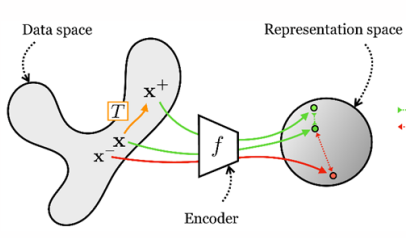
\includegraphics[width=0.6\textwidth]{images/Representation Learning.png}
  \caption{\centering High-level picture of representation learning.
           The encoder $f_\theta$ maps a raw input $\mathbf{x}$ to
           a structured latent vector $\mathbf{z}$, which is then
           used for a downstream task such as classification or
           fairness-aware prediction.}
  \label{fig:repr_learning}
\end{figure}

% , , , , , , , , , , , , , , , , , , , , , , 
\section{Disentangled Representation Learning}
\label{sec:disentangled}
% , , , , , , , , , , , , , , , , , , , , , , 

Standard representation learning makes no assumption about the
\emph{structure} of the latent space.  \emph{Disentangled}
representation learning imposes the additional constraint that
different dimensions (or subspaces) of $\mathbf{z}$ capture
statistically independent generative factors of the data
\cite{bengio2013, higgins2017, kim2018}.

Formally, if the data is generated by $K$ independent factors
$v_1, v_2, \ldots, v_K$, a disentangled encoder should produce
a latent vector $\mathbf{z} = [z_1, z_2, \ldots, z_K]$ such that
\[
  q_\Phi(z_1, z_2, \ldots, z_K)
  \;\approx\;
  \prod_{k=1}^{K} q_\Phi(z_k),
\]
i.e., the joint latent distribution factorises into independent
marginals.  This is precisely the condition that Total Correlation
(Eq.~\ref{eq:total_correlation}) is zero.

\begin{figure}[htbp]
  \centering
  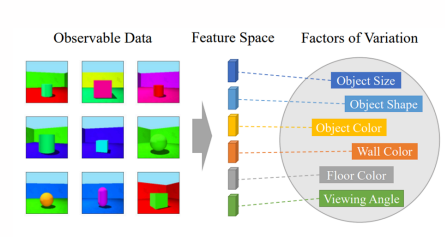
\includegraphics[width=0.8\textwidth]{images/Disentangled.png}
  \caption{Illustration of disentangled representation learning showing mapping from observable data to feature space and factors of variation.}
  \label{fig:disentangled}
\end{figure}
\noindent\textbf{Why does disentanglement matter for fairness?}
If a latent space is properly disentangled, one can isolate and
\emph{remove} the subspace that encodes sensitive demographic
information before passing representations to a downstream
classifier, achieving fairness without sacrificing
task-relevant information.

% , , , , , , , , , , , , , , , , , , , , , , 
\section{Autoencoders}
\label{sec:autoencoders}
% , , , , , , , , , , , , , , , , , , , , , , 

An \emph{autoencoder} is a neural network trained to reconstruct
its input through a bottleneck layer.  It consists of two
components:

\begin{itemize}
  \item \textbf{Encoder} $E_\theta: \mathcal{X} \to \mathcal{Z}$
        compresses the input $\mathbf{x}$ into a latent code
        $\mathbf{z} = E_\theta(\mathbf{x})$.
  \item \textbf{Decoder} $G_\phi: \mathcal{Z} \to \mathcal{X}$
        reconstructs the input as
        $\hat{\mathbf{x}} = G_\phi(\mathbf{z})$.
\end{itemize}

Training minimises reconstruction loss, typically mean-squared error:
\begin{equation}
  \mathcal{L}_{\mathrm{AE}}
  \;=\; \mathbb{E}_{\mathbf{x}}\!\left[
        \bigl\|\mathbf{x} - G_\phi(E_\theta(\mathbf{x}))\bigr\|^2
        \right].
  \label{eq:ae_loss}
\end{equation}
The bottleneck forces the encoder to discard redundant information
and retain only the structure necessary for reconstruction.

\begin{figure}[htbp]
  \centering
  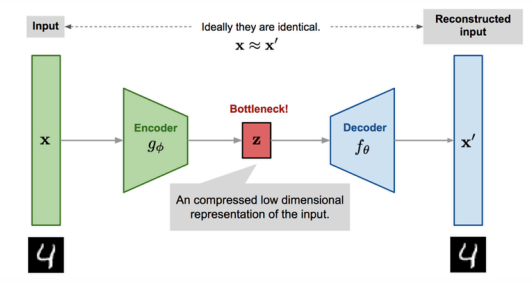
\includegraphics[width=0.8\textwidth]{images/Autoencoder.png}
  \caption{Autoencoder architecture: the encoder $g_\phi$ maps input $\mathbf{x}$ to a low-dimensional latent representation $\mathbf{z}$ (bottleneck), and the decoder $f_\theta$ reconstructs the input as $\mathbf{x'} \approx \mathbf{x}$.}
  \label{fig:autoencoder}
\end{figure}

% , , , , , , , , , , , , , , , , , , , , , , 
\section{Variational Autoencoders (VAE)}
\label{sec:vae}
% , , , , , , , , , , , , , , , , , , , , , , 

A \emph{Variational Autoencoder} (VAE) \cite{kingma2014} is a
probabilistic generative model that frames encoding and decoding
as Bayesian inference.  Instead of mapping an input to a single
point in latent space, the encoder outputs a \emph{distribution}:
\[
  q_\Phi(\mathbf{z}|\mathbf{x})
  = \mathcal{N}\!\bigl(\boldsymbol{\mu}_{q_\Phi}(\mathbf{x}),\;
                        \boldsymbol{\sigma}^2_{q_\Phi}(\mathbf{x})\bigr),
\]
where $\boldsymbol{\mu}$ and $\boldsymbol{\sigma}$ are output by
the encoder network with parameters $\Phi$.  The decoder models
$p_\Theta(\mathbf{x}|\mathbf{z})$.

\noindent\textbf{Reparameterisation trick.}
To enable gradient-based optimisation through a stochastic node,
we sample
\begin{equation}
  \mathbf{z} = \boldsymbol{\mu}_{q_\Phi}(\mathbf{x})
               + \boldsymbol{\sigma}_{q_\Phi}(\mathbf{x}) \odot
               \boldsymbol{\epsilon}, \qquad
  \boldsymbol{\epsilon} \sim \mathcal{N}(\mathbf{0}, \mathbf{I}),
  \label{eq:reparam}
\end{equation}
which moves the randomness outside the computational graph.

\noindent\textbf{Training objective.}
The VAE is trained by maximising the ELBO
(Eq.~\ref{eq:elbo}), which can be written explicitly as:
\begin{equation}
  \mathcal{L}_{\mathrm{VAE}}
  = \sum_{i=1}^{N}
    \Bigl[
      \mathbb{E}_{q_\Phi(\mathbf{z}|\mathbf{x}_i)}\!
      \bigl[\log p_\Theta(\mathbf{x}_i|\mathbf{z})\bigr]
      -
      D_{\mathrm{KL}}\!\bigl(
        q_\Phi(\mathbf{z}|\mathbf{x}_i)\,\|\, p(\mathbf{z})
      \bigr)
    \Bigr].
  \label{eq:vae_loss}
\end{equation}

\noindent\textbf{Extensions for disentanglement.}
$\beta$-VAE \cite{higgins2017} up-weights the KL term by a
hyperparameter $\beta > 1$ to encourage greater disentanglement at
the cost of reconstruction quality.
FactorVAE \cite{kim2018} and $\beta$-TCVAE \cite{chen2018} instead
minimise Total Correlation directly (Eq.~\ref{eq:total_correlation}),
yielding better disentanglement without degrading reconstruction.

% , , , , , , , , , , , , , , , , , , , , , , 
\section{Adversarial Learning}
\label{sec:adversarial}
% , , , , , , , , , , , , , , , , , , , , , , 

\emph{Adversarial learning} is a training paradigm in which two
model components compete in a minimax game, each driving the other
towards a more useful solution \cite{goodfellow2014}.

\subsection{Generative Adversarial Networks (GANs)}

In the canonical GAN setup, a generator $G$ learns to produce
synthetic samples that fool a discriminator $D$, while $D$ learns to
distinguish real from fake:
\begin{equation}
  \min_{G}\;\max_{D}\;
  \mathbb{E}_{\mathbf{x}\sim p_{\mathrm{data}}}\!\bigl[\log D(\mathbf{x})\bigr]
  + \mathbb{E}_{\mathbf{z}\sim p(\mathbf{z})}\!\bigl[\log(1 - D(G(\mathbf{z})))\bigr].
  \label{eq:gan}
\end{equation}
At equilibrium, $G$ produces samples from $p_{\mathrm{data}}$ and $D$
cannot distinguish real from generated samples.

\begin{figure}[htbp]
  \centering
  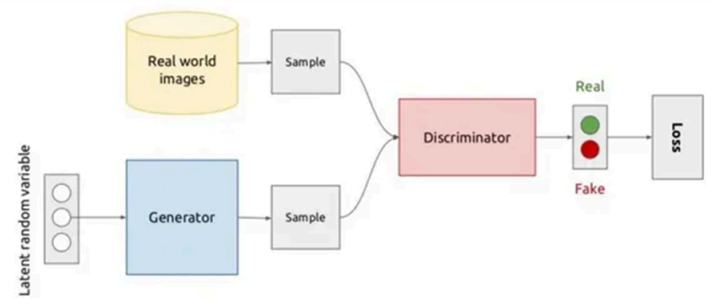
\includegraphics[width=0.85\textwidth]{images/Adversarial .png}
  \caption{Generative Adversarial Network (GAN): the generator maps latent variables to synthetic samples, while the discriminator distinguishes between real and generated data, providing a training signal via adversarial loss.}
  \label{fig:gan}
\end{figure}

\subsection{Adversarial Debiasing}
\label{subsec:adv_debiasing}

In fair representation learning, adversarial networks serve a
different role.  A \emph{predictor} $P$ is trained to predict
a target label $y$ from a representation $\mathbf{z}$, while an
\emph{adversary} $A$ attempts to predict the sensitive attribute
$s$ from the same $\mathbf{z}$.  The encoder is then trained to
\emph{fool the adversary}:
\begin{equation}
  \min_{E,P}\;\max_{A}\;
  \mathcal{L}_{\mathrm{pred}}(P(E(\mathbf{x})),\, y)
  \;-\; \lambda\,\mathcal{L}_{\mathrm{adv}}(A(E(\mathbf{x})),\, s).
  \label{eq:adv_debias}
\end{equation}
The negative sign on the adversarial loss means the encoder
\emph{maximises} the adversary's error—equivalently, it removes
sensitive information from $\mathbf{z}$.

\noindent\textbf{Gradient Reversal Layer (GRL).}
A practical implementation of Eq.~\ref{eq:adv_debias} uses a
Gradient Reversal Layer (GRL) \cite{ganin2016}.  During
the forward pass, GRL acts as the identity; during
back-propagation, it negates the gradient, automatically
implementing the minimax objective without alternating optimisation:
\begin{equation}
  \mathrm{GRL}(\mathbf{z}) = \mathbf{z}, \qquad
  \frac{\partial\,\mathrm{GRL}(\mathbf{z})}{\partial\,\mathbf{z}}
  = -\lambda_{\mathrm{grl}}\,\mathbf{I}.
  \label{eq:grl}
\end{equation}

% , , , , , , , , , , , , , , , , , , , , , , 
\section{Fractional Fourier Transform (FrFT)}
\label{sec:frft}
% , , , , , , , , , , , , , , , , , , , , , , 

The classical Fourier transform maps a signal from the time domain
to the frequency domain.  The \emph{Fractional Fourier Transform}
(FrFT) \cite{ozaktas2001} is a generalisation parameterised by a
rotation order $\alpha \in [0,1]$, interpolating continuously
between the time ($\alpha=0$) and frequency ($\alpha=1$) domains:
\begin{equation}
  \mathcal{F}_\alpha[f](u)
  = \int_{-\infty}^{\infty} f(t)\,K_\alpha(t,u)\,\mathrm{d}t,
  \label{eq:frft}
\end{equation}
where the kernel is
\[
  K_\alpha(t, u)
  = A_\alpha\,
    \exp\!\bigl(
      i\pi(t^2 \cot\alpha - 2tu\csc\alpha + u^2 \cot\alpha)
    \bigr), \qquad
  A_\alpha = \sqrt{1 - i\cot\alpha}.
\]
Deepfake generation pipelines introduce subtle frequency artefacts
that are more discriminative in intermediate spatial–frequency
domains than in either the pure spatial or pure frequency domain
\cite{liu2021}.  By selecting $\alpha$ between 0 and 1, the FrFT
exposes these artefacts while reducing reliance on demographic
appearance features (skin tone, facial structure) that dominate
the spatial domain.

\begin{figure}[htbp]
  \centering
  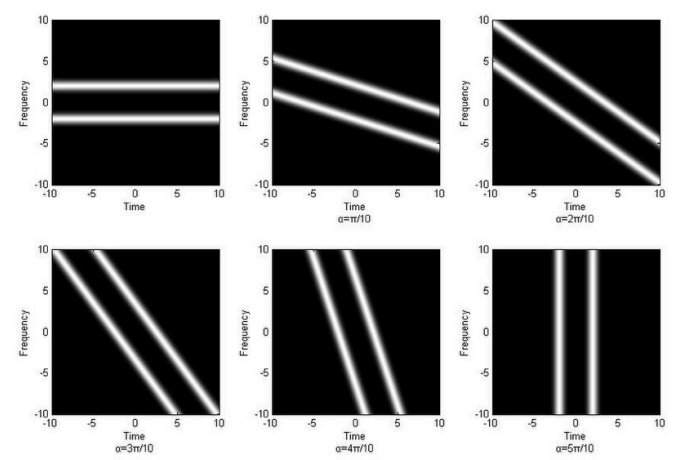
\includegraphics[width=\textwidth]{images/FRFT.png}
  \caption{Fractional Fourier Transform (FRFT) representations at different fractional orders $\alpha$, showing the rotation of signal energy in the time-frequency plane.}
  \label{fig:frft}
\end{figure}

% , , , , , , , , , , , , , , , , , , , , , , 
\section{Fairness Concepts in Machine Learning}
\label{sec:fairness_concepts}
% , , , , , , , , , , , , , , , , , , , , , , 

Before defining evaluation metrics, we establish the terminology
used throughout this report.

\begin{itemize}
  \item \textbf{Target attribute} ($y_t$): the label the model is
        trained to predict (e.g., ``attractive'', ``real/fake'').
  \item \textbf{Protected (sensitive) attribute} ($y_p$):
        a demographic characteristic (e.g., gender, race, age)
        with respect to which the model should \emph{not}
        discriminate.
  \item \textbf{Group fairness}: equal treatment of pre-specified
        demographic groups.
  \item \textbf{Individual fairness}: similar individuals receive
        similar predictions.
\end{itemize}

Let $\hat{Y}$ denote the model's prediction, $Y$ the ground truth
label ($Y=1$ positive, $Y=0$ negative), and $G \in \{g_0, g_1\}$
the protected group membership.  Define:
\begin{align*}
  \mathrm{TPR}_g &= \Pr(\hat{Y}=1 \mid Y=1,\, G=g),
  \quad\text{(True Positive Rate for group }g)\\
  \mathrm{TNR}_g &= \Pr(\hat{Y}=0 \mid Y=0,\, G=g),
  \quad\text{(True Negative Rate for group }g)\\
  \mathrm{FPR}_g &= \Pr(\hat{Y}=1 \mid Y=0,\, G=g).
  \quad\text{(False Positive Rate for group }g)
\end{align*}

% , , , , , , , , , , , , , , , , , , , , , , 
\section{Evaluation Metrics}
\label{sec:eval_metrics}
% , , , , , , , , , , , , , , , , , , , , , , 

\subsection{Equal Opportunity}
\label{subsec:equal_opp}

\emph{Equal Opportunity} \cite{hardt2016} requires that the
True Positive Rate be equal across protected groups.  A model
satisfies equal opportunity if subjects who \emph{deserve} a
positive outcome are equally likely to receive it, regardless
of group membership.  It is measured as:
\begin{equation}
  \Delta_{\mathrm{EO}}
  = \bigl|\mathrm{TPR}_{g_0} - \mathrm{TPR}_{g_1}\bigr|.
  \label{eq:equal_opp}
\end{equation}
A value of $\Delta_{\mathrm{EO}} = 0$ indicates perfect equal
opportunity; \emph{lower is better}.

\subsection{Equalized Odds}
\label{subsec:equalized_odds}

\emph{Equalized Odds} \cite{hardt2016} is a stricter criterion:
the model must achieve equal TPR \emph{and} equal TNR across
groups simultaneously.  This ensures both that qualified
candidates are equally recognised and that unqualified ones are
equally rejected:
\begin{equation}
  \Delta_{\mathrm{EOdd}}
  = \frac{1}{2}\Bigl(
      \bigl|\mathrm{TPR}_{g_0} - \mathrm{TPR}_{g_1}\bigr|
      +
      \bigl|\mathrm{TNR}_{g_0} - \mathrm{TNR}_{g_1}\bigr|
    \Bigr).
  \label{eq:equalized_odds}
\end{equation}
Again, \emph{lower is better}.  The relationship between these
two metrics is: a model satisfying equalized odds also satisfies
equal opportunity, but not vice versa.

\subsection{Standard Accuracy}
\label{subsec:accuracy}

Standard accuracy is the fraction of correctly classified samples:
\begin{equation}
  \mathrm{Acc}
  = \frac{\text{Number of correct predictions}}
         {\text{Total number of predictions}}.
  \label{eq:accuracy}
\end{equation}
While essential for gauging utility, accuracy alone is a misleading
fairness proxy.  On an imbalanced dataset biased towards one
demographic group, a model can achieve high accuracy while
systematically harming an underrepresented group.

\subsection{Equalized Accuracy}
\label{subsec:equalized_acc}

To address the limitations of standard accuracy on skewed test
distributions, the README paper \cite{park2020} introduces
\emph{Equalized Accuracy}, which averages TPR and TNR across
both groups equally:
\begin{equation}
  \mathrm{EAcc}
  = \frac{1}{4}\Bigl(
      \mathrm{TPR}_{g_0} + \mathrm{TNR}_{g_0}
      + \mathrm{TPR}_{g_1} + \mathrm{TNR}_{g_1}
    \Bigr).
  \label{eq:equalized_acc}
\end{equation}
Because each group contributes equally regardless of its size in
the dataset, Equalized Accuracy is a more reliable indicator of
a model's generalisation across the population.

\subsection{FPR-Based Fairness Metrics for Deepfake Detection}
\label{subsec:fpr_metrics}

In the context of deepfake detection, where real faces vastly
outnumber deepfakes in practice, \emph{False Positive Rate}
disparities can have severe societal consequences: real individuals
being misclassified as deepfakes and subjected to unjust scrutiny
\cite{ju2024}.  Three metrics capture this:

\begin{enumerate}
  \item \textbf{FPR Gap} ($G_{\mathrm{FPR}}$): maximum pairwise
        difference in FPR across demographic groups:
        \begin{equation}
          G_{\mathrm{FPR}}
          = \max_{g,g' \in \mathcal{G}}
            \bigl|\mathrm{FPR}_g - \mathrm{FPR}_{g'}\bigr|.
          \label{eq:fpr_gap}
        \end{equation}

  \item \textbf{Equal FPR} ($F_{\mathrm{FPR}}$): summed absolute
        difference between each group's FPR and the overall FPR:
        \begin{equation}
          F_{\mathrm{FPR}}
          = \sum_{g \in \mathcal{G}}
            \left|
              \frac{\sum_i \mathbf{1}[\hat{Y}_i=1,\,G_i=g,\,Y_i=0]}
                   {\sum_i \mathbf{1}[G_i=g,\,Y_i=0]}
              -
              \frac{\sum_i \mathbf{1}[\hat{Y}_i=1,\,Y_i=0]}
                   {\sum_i \mathbf{1}[Y_i=0]}
            \right|.
          \label{eq:equal_fpr}
        \end{equation}

  \item \textbf{Fair Equalized Odds} ($F_{\mathrm{EO}}$):
        extends Equal FPR to both positive and negative classes:
        \begin{equation}
          F_{\mathrm{EO}}
          = \sum_{g \in \mathcal{G}} \sum_{q \in \{0,1\}}
            \left|
              \frac{\sum_i \mathbf{1}[\hat{Y}_i=1,\,G_i=g,\,Y_i=q]}
                   {\sum_i \mathbf{1}[G_i=g,\,Y_i=q]}
              -
              \frac{\sum_i \mathbf{1}[\hat{Y}_i=1,\,Y_i=q]}
                   {\sum_i \mathbf{1}[Y_i=q]}
            \right|.
          \label{eq:fair_eo}
        \end{equation}
\end{enumerate}
For all three metrics, lower values indicate greater fairness.

\subsection{Summary of Metrics}
\label{subsec:metrics_summary}

Table~\ref{tab:metrics_summary} summarises all evaluation metrics,
their target conditions, and the direction of improvement.
\begin{table}[!htbp]
  \centering
  \caption{Summary of fairness and utility evaluation metrics used
           in this report.  All fairness metrics are minimised;
           accuracy metrics are maximised.}
  \label{tab:metrics_summary}
  \small
  \begin{tabular}{llll}
    \toprule
    \textbf{Metric} & \textbf{Symbol} & \textbf{Condition checked}
                    & \textbf{Better} \\
    \midrule
    Equal Opportunity   & $\Delta_{\mathrm{EO}}$     & TPR equal across groups    & $\downarrow$ \\
    Equalized Odds      & $\Delta_{\mathrm{EOdd}}$   & TPR \& TNR equal           & $\downarrow$ \\
    Standard Accuracy   & $\mathrm{Acc}$             & Overall correctness        & $\uparrow$   \\
    Equalized Accuracy  & $\mathrm{EAcc}$            & Balanced group accuracy    & $\uparrow$   \\
    FPR Gap             & $G_{\mathrm{FPR}}$         & Max FPR spread             & $\downarrow$ \\
    Equal FPR           & $F_{\mathrm{FPR}}$         & FPR parity per group       & $\downarrow$ \\
    Fair Equalized Odds & $F_{\mathrm{EO}}$          & TPR \& FPR parity          & $\downarrow$ \\
    AUC-ROC             & AUC                        & Ranking quality            & $\uparrow$   \\
    \bottomrule
  \end{tabular}
\end{table}

% , , , , , , , , , , , , , , , , , , , , , , 
\section{Key Deep Learning Architectures Used in Fair AI}
\label{sec:architectures}
% , , , , , , , , , , , , , , , , , , , , , , 

Table~\ref{tab:model_summary} provides a concise comparison of the
core neural-network models referenced throughout this report.
\begin{table}[!htbp]
  \centering
  \caption{Key model architectures referenced in the fairness-in-AI
           literature covered in this report.}
  \label{tab:model_summary}
  \small
  \begin{tabular}{p{2.4cm}p{3.2cm}p{3.5cm}p{3.5cm}}
    \toprule
    \textbf{Model} & \textbf{Core idea} & \textbf{Strength}
                   & \textbf{Limitation} \\
    \midrule
    VAE \cite{kingma2014}
      & Probabilistic encoder–decoder with Gaussian latent prior
      & Smooth, generative latent space
      & No explicit control over which factors are captured \\
    $\beta$-VAE \cite{higgins2017}
      & Up-weight KL term by $\beta$
      & Encourages disentanglement
      & Hurts reconstruction at high $\beta$ \\
    FactorVAE \cite{kim2018}
      & Minimise Total Correlation via discriminator
      & Better disentanglement than $\beta$-VAE
      & Requires an additional discriminator \\
    FFVAE \cite{creager2019}
      & Disentangle sensitive vs.\ non-sensitive latents
      & Fairness-focused VAE
      & Sensitive latents leak target attribute info \\
    FD-VAE \cite{park2020}
      & Three-way split: TAL, PAL, MAL + decorrelation loss
      & Explicitly decorrelates attributes
      & Requires target \& protected attribute labels \\
    Adversarial Autoencoder
      & GRL to strip demographic info from $\mathbf{z}$
      & Architecture-level fairness
      & Adversarial training instability \\
    FAIR-FRFT (ours)
      & FrFT + adversarial autoencoder + CVaR
      & Frequency-domain fairness
      & Higher computational cost \\
    \bottomrule
  \end{tabular}
\end{table}

% , , , , , , , , , , , , , , , , , , , , , , 
\section{Chapter Summary}
\label{sec:ch2_summary}
% , , , , , , , , , , , , , , , , , , , , , , 

This chapter introduced the mathematical and conceptual vocabulary
needed to follow the technical discussions in subsequent chapters.

\begin{itemize}
  \item \textbf{Mathematical tools}: KL divergence, Total
        Correlation, mutual information, ELBO, and CVaR provide
        the optimisation-theoretic backbone for fair
        representation learning.
  \item \textbf{Architectures}: Autoencoders, VAEs, and adversarial
        networks are the primary building blocks; disentanglement
        methods extend them to produce interpretable, attribute-separable
        latent spaces.
  \item \textbf{FrFT}: Offers a hybrid spatial–frequency domain
        well-suited to capturing deepfake artefacts that are less
        correlated with demographic features.
  \item \textbf{Evaluation metrics}: Equal Opportunity,
        Equalized Odds, Equalized Accuracy, and FPR-based metrics
        together give a multi-dimensional picture of fairness;
        no single metric suffices.
\end{itemize}